\section{InterProScan as Supporting Evidence for Predicted Genes}\label{section:interproscan}

Pfam hits from InterProScan analysis are presented in
Figure~\ref{fig:ips-counts} and Table~\ref{table:ips-pfam}, from
which we can identify one major trend. In general, roughly 73\-76\% of
proteins predicted by Braker2, GeneMark and RefSeq contain a match to
a Pfam entry, except in the case of \textit{T. harzianum}, which
reports a considerably lower proportion of genes with Pfam matches in
the RefSeq dataset. Why the proportion of RefSeq proteins with Pfam
matches in \textit{T. harzianum} is so low is unknown. This is
promising performance for the gene finders as the RefSeq annotations
demonstrate similar proportions of Pfam hits to predicted
proteins. The total counts may be deceiving however, as predictions
from Braker2 may result in more than one protein product per gene,
whereas in the case of GeneMark, only one protein is produced per gene
model. From visual inspection of Pfam hits mapped back to the
references it appears that, in general, when gene finders agree that a
gene is present, InterProScan reports the same Pfam match in all three
predictions. An example of agreement between Braker2, GeneMark, RefSeq
and InterProScan is shown in Figure ~\ref{fig:basic-agree}. It is
important to note that the position of the Pfam match in IGV does not
indicate the true position of the Pfam match in the gene, but provides
an indication of the presence of Pfam matches. Pfam matches are offset
from the start of the gene based on the start and end position of the
Pfam match in the protein sequence. For example, if a Pfam match has a
start position 10 amino acids into the protein sequence, the
corresponding start position in the resulting GFF is 10bp downstream
from the start of the gene.

\begin{figure}
  \centering
  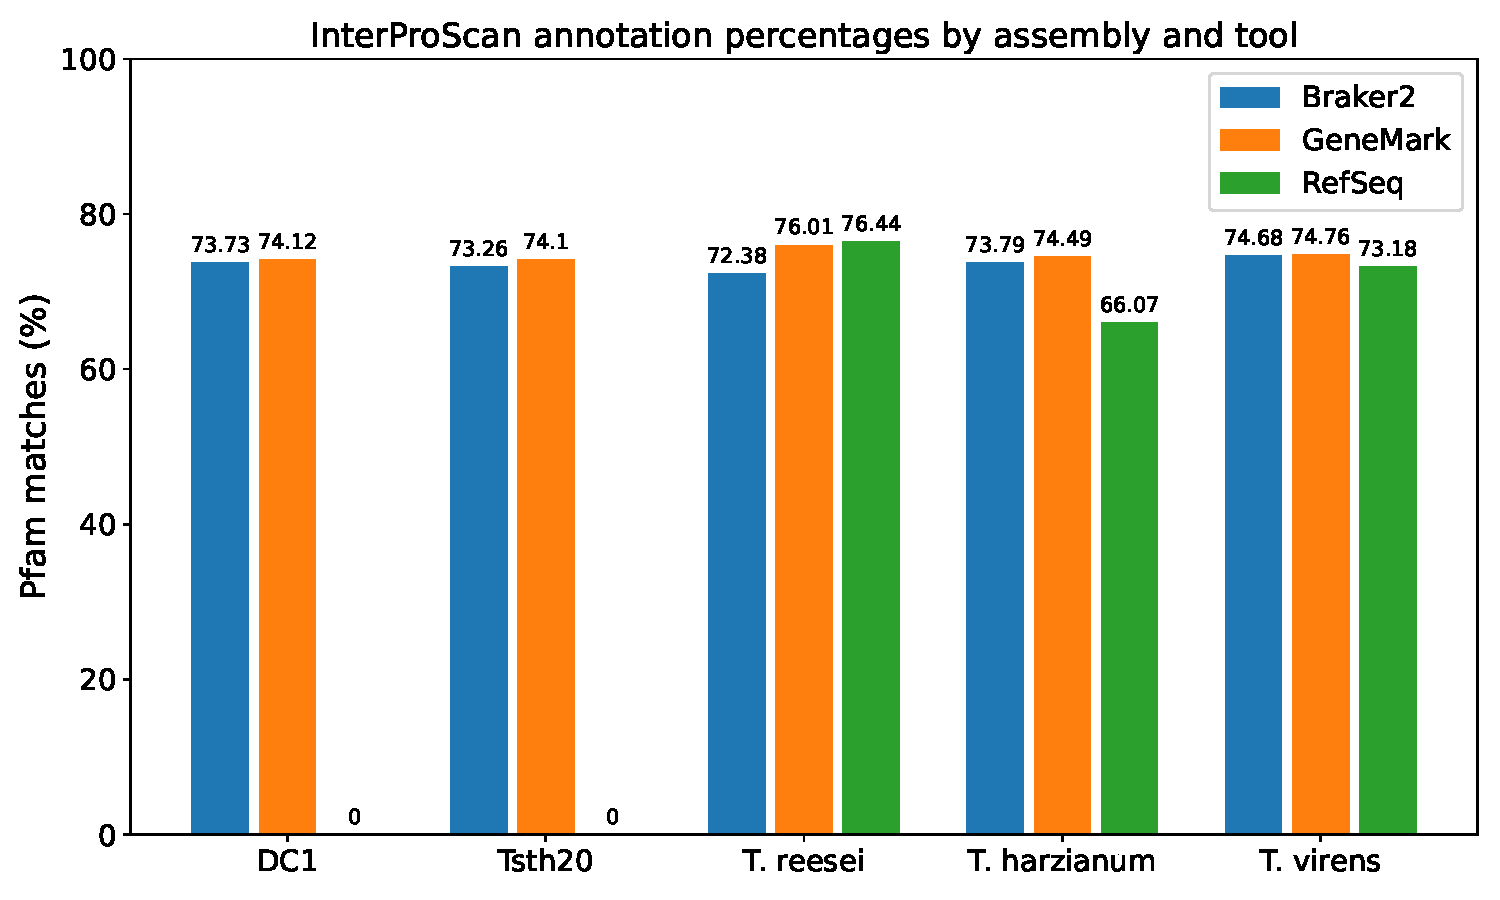
\includegraphics[width=0.90\textwidth]{figures/interproscan-barplot.pdf}
  \caption[Percentage of proteins with Pfam matches]{Bar plot showing the percentage of predicted proteins with Pfam matches from InterProScan for each gene finder across all \textit{Trichoderma} genome assemblies. For DC1 and Tsth20, RefSeq annotations are not available, so their values are set to 0.}\label{fig:ips-counts}
\end{figure}

\begin{table}[h!]
  \centering
  \begin{tabular}{|c|c|c|c|}
    \hline
    Assembly & Braker2 (\%) & GeneMark (\%) & RefSeq (\%) \\ \hline
    DC1 & 73.73 & 74.12 & N/A \\ \hline
    Tsth20 & 73.26 & 74.10 & N/A \\ \hline
    \textit{T. reesei} & 72.38 & 76.01 & 76.44 \\ \hline
    \textit{T. harzianum} & 73.79 & 74.49 & 66.07 \\ \hline
    \textit{T. virens} & 74.68 & 74.76 & 73.18 \\ \hline
  \end{tabular}
  \caption[InterProScan Pfam Evidence]{Table showing the fractions of predicted
    genes with Pfam annotations from InterProScan as a percent}\label{table:ips-pfam}
\end{table}

% DC1: 73.73\%, 74.12\%, N/A
% Tsth20: 73.26\%, 74.10\%, N/A
% \textit{T. reesei}: 72.38\%, 76.01\%, 76.44\%
% \textit{T. harzianum}: 73.79\%, 74.49\%, 66.07\%
% \textit{T. virens}: 74.68\%, 74.76\%, 73.18\%

%    DC1 & $100\times(\frac{10676}{14479})=73.73\%$ & $100\times(\frac{8416}{11354})=74.12\%$ & N/A \\ \hline
%    Tsth20 & $100\times(\frac{11389}{15546})=73.26\%$ & $100\times(\frac{9168}{12373})=74.10\%$ & N/A \\ \hline
%    \textit{T. reesei} & $100\times(\frac{8471}{11704})=72.38\%$ & $100\times(\frac{6990}{9196})=76.01\%$ & $100\times(\frac{6964}{9111})=76.44\%$ \\ \hline
%    \textit{T. harzianum} & $100\times(\frac{11370}{15408})=73.79\%$ & $100\times(\frac{9061}{12164})=74.49\%$ & $100\times(\frac{9293}{14065})=66.07\%$ \\ \hline
%    \textit{T. virens} & $100\times(\frac{11249}{15062})=74.68\%$ & $100\times(\frac{8871}{11866})=74.76\%$ & $100\times(\frac{9062}{12383})=73.18\%$ \\ \hline

\begin{figure}[h!]
  \centering
  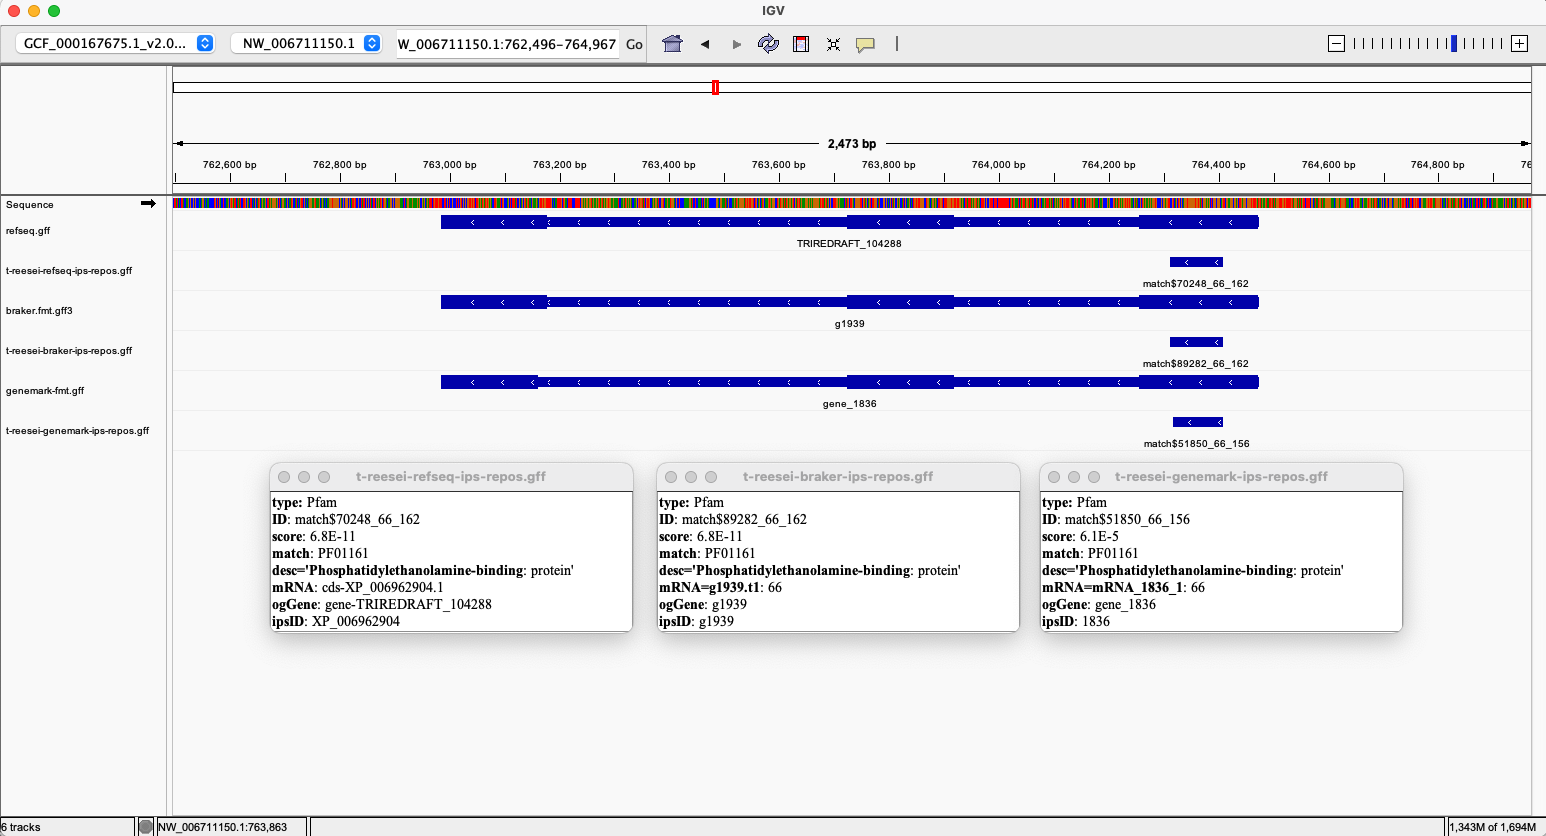
\includegraphics[width=\textwidth]{figures/igv/ips-basic-agree.png}
  \caption[Agreeing Pfam matches]{An IGV capture showing complete
    agreement between gene finders for both gene model and protein
    Pfam hits. The longer segments are predicted genes and the smaller
    segments are annotated Pfam matches, all with agreeing start and
    stop positions. The description in each sub-window indicates the
    agreeing Pfam annotations.}\label{fig:basic-agree}
\end{figure}

While cases of complete agreement are abundant, cases of disagreement
also exist and in strange forms. In many cases, while the gene finders
agree on the presence of a gene, only the RefSeq protein product
contains a match to the Pfam database. Why this may be the case is
unclear, and may warrant further investigation. There are also many
cases in which InterProScan reports the same Pfam hits for individual
proteins, but the gene models in the region do not agree. There are
even cases such as the region shown in Figure
~\ref{fig:agree-bizarre2}, where Braker2 and GeneMark agree that two
genes and their associated proteins and Pfam matches are separate, but
RefSeq only reports one gene with multiple Pfam hits. There are also
several cases where two tools are in agreement with proteins
containing Pfam hits while another is not. Even more interesting are
cases such as the one shown in Figure~\ref{fig:ips-no-refseq}, in
which Braker2 and GeneMark predictions contain Pfam matches while
RefSeq does not report a gene at all. This may be the due to
experimental data used in the RefSeq training process or a result of
curation. Regardless of the tool, these cases demonstrate well that
gene finders are not always in agreement even on well known proteins,
to the point that predictions are not present even though protein
products from other gene finders contain known Pfam matches.

\begin{figure}[h!]
  \centering
  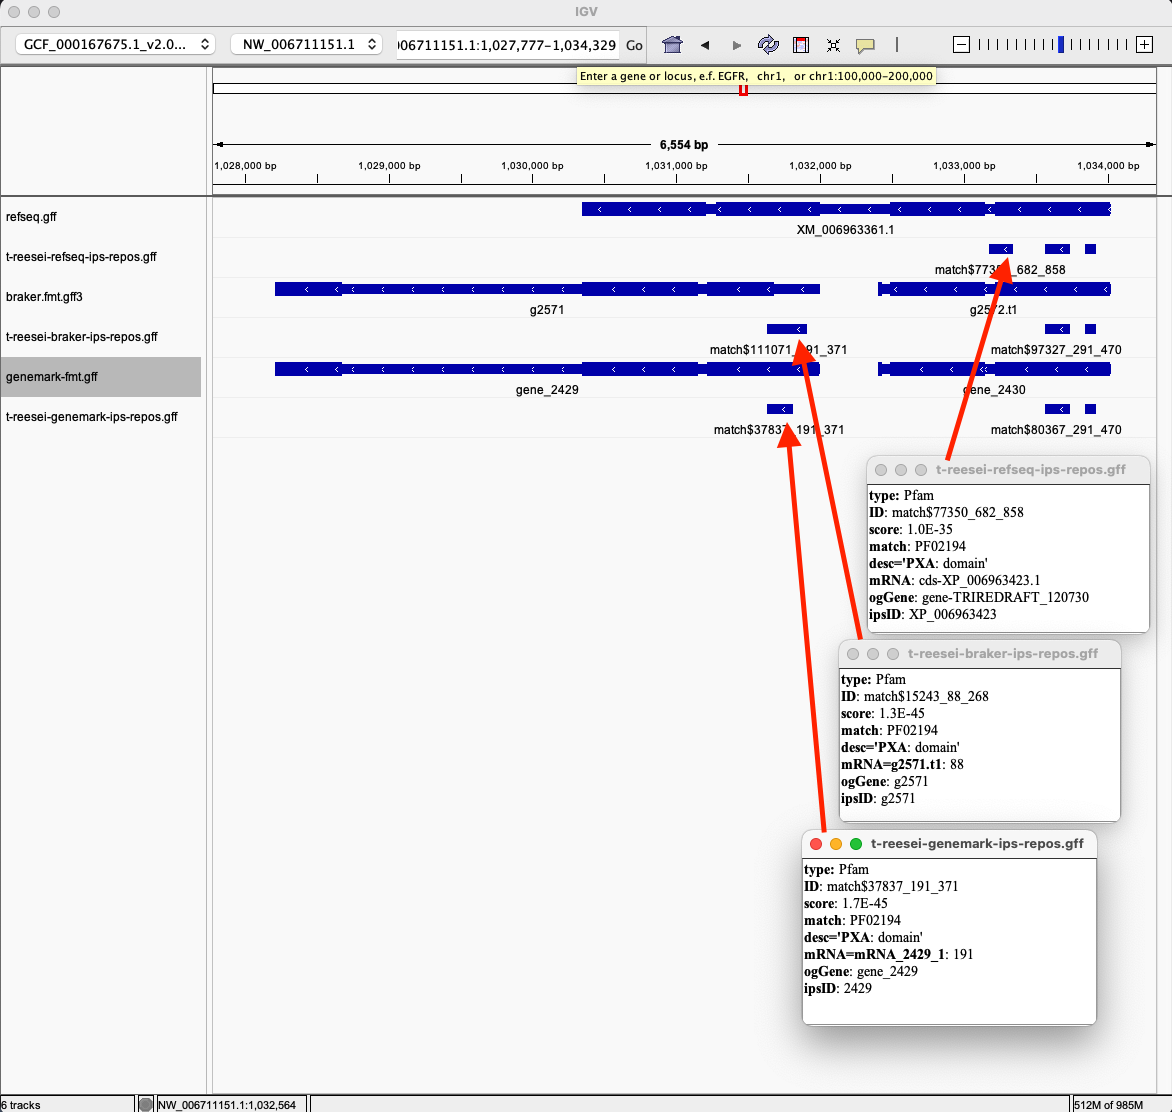
\includegraphics[width=\textwidth]{figures/igv/ips-model-disagree2.png}
  \caption[Split Pfam matches]{An IGV capture showing Braker2 and
    GeneMark reporting two genes and their resulting proteins and
    Pfam hits as separate, while RefSeq reports one gene, one protein
    and three Pfam matches.}\label{fig:agree-bizarre2}
\end{figure}

\begin{figure}
  \centering
  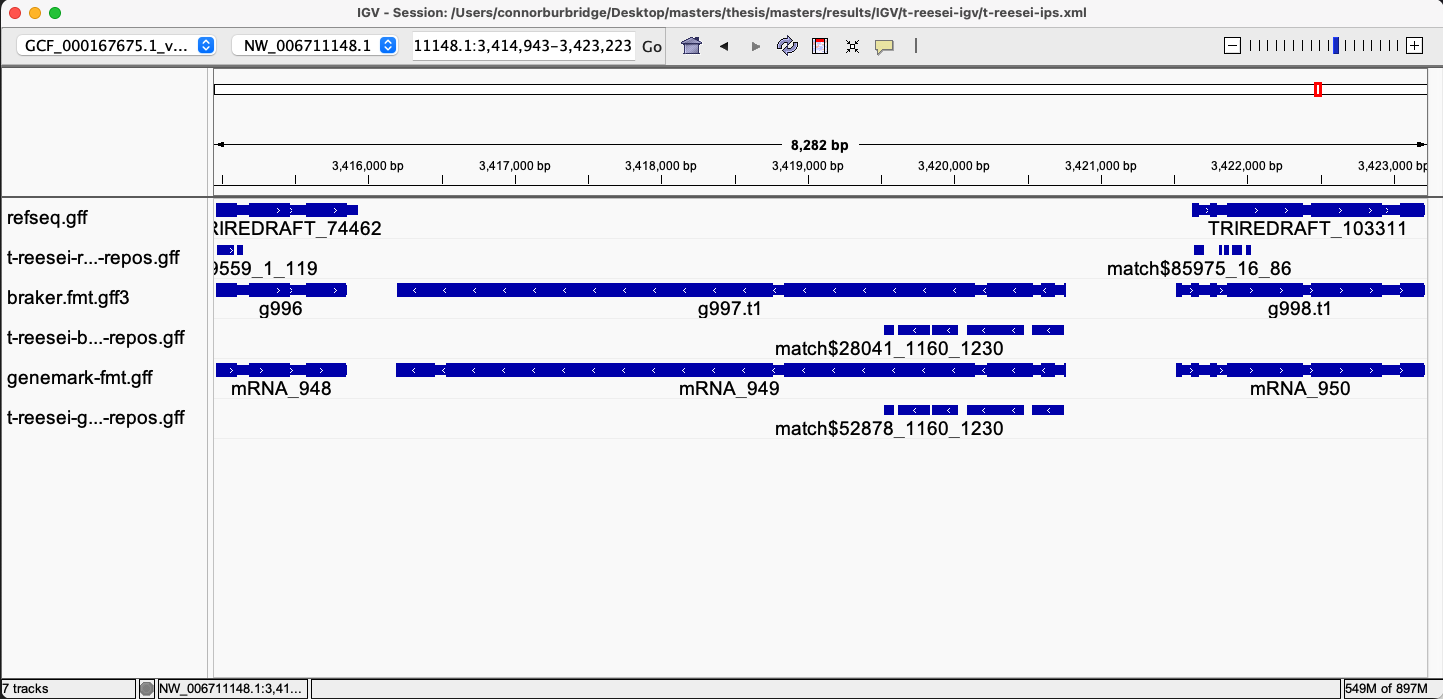
\includegraphics[width=\textwidth]{figures/igv/ips-braker-genemark-norefseq.png}
  \caption[RefSeq absence with IPS evidence]{An IGV capture showing a
    scenario where GeneMark and Braker2 agree on a gene model with
    supporting Pfam evidence and RefSeq does not report any gene.}\label{fig:ips-no-refseq}
\end{figure}

In summary, the protein products from Braker2 and GeneMark predictions
do contain matches to the Pfam database. The proportions of matches to
total proteins are similar to that of the RefSeq annotation, sitting
between 65 and 75 percent. While Pfam hits to Braker2, GeneMark and
RefSeq proteins generally agree, we observe regions in which there
is disagreement in several forms.
